%==============================================================================
% Document header
%==============================================================================
\documentclass[a4paper,11pt]{article}

% Color package
\usepackage[usenames,dvipsnames]{color}

% Hyperrefs
\usepackage[
  colorlinks = true,
  linkcolor  = Mahogany,
  citecolor  = Mahogany,
  urlcolor   = blue,
]{hyperref}

\usepackage{graphicx}
\usepackage{rotating}
\usepackage{multirow}

\usepackage{longtable}

% Header and footer customization
\usepackage{fancyhdr}
\pagestyle{fancy}
\fancyhead[L]{\nouppercase{\leftmark}}
\fancyhead[R]{} 
\renewcommand{\footrulewidth}{0.4pt}

%==============================================================================
% Start of document
%==============================================================================
\begin{document}

%------------------------------------------------------------------------------
% Title
%------------------------------------------------------------------------------
\begin{titlepage}

\vspace*{3cm}

\noindent{\LARGE \textbf{I$^2$C Slave Core}}

\noindent \rule{\textwidth}{.1cm}

\hfill\today

\vspace*{3cm}

\begin{figure}[h]
  
\includegraphics[height=3cm]{fig/cern-logo}
  \hfill
  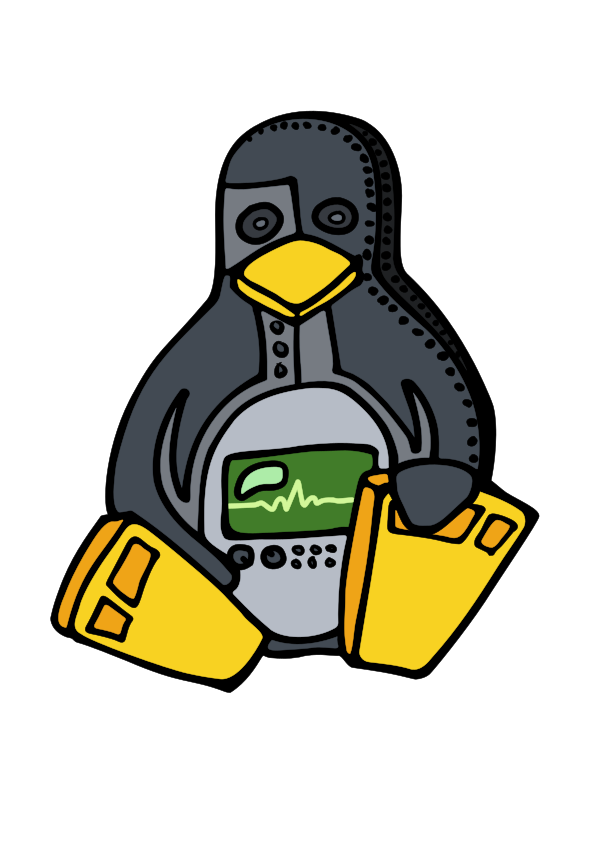
\includegraphics[height=3cm]{fig/ohwr-logo}
\end{figure}

\vfill

\noindent {\Large \textbf{Theodor-Adrian Stana (CERN/BE-CO-HT)}}

\noindent \rule{\textwidth}{.05cm}

\end{titlepage}


%------------------------------------------------------------------------------
% Revision history
%------------------------------------------------------------------------------
\thispagestyle{empty}
\section*{Revision history}

\centerline
{
  \begin{tabular}{l c p{.6\textwidth}}
  \hline
  \multicolumn{1}{c}{\textbf{Date}} & \multicolumn{1}{c}{\textbf{Version}} & \multicolumn{1}{c}{\textbf{Change}} \\
  \hline
  26-06-2013 & 0.01 & First draft \\
  28-10-2013 & 0.02 & Changed PDF link colors \\
  \hline
  \end{tabular}
}

%------------------------------------------------------------------------------
% Generate TOC and pagebreak after it
%------------------------------------------------------------------------------
\pagebreak
\pagenumbering{roman}
\setcounter{page}{1}
\tableofcontents

%------------------------------------------------------------------------------
% List of figs, tables, abbrevs
%------------------------------------------------------------------------------
\pagebreak
\listoffigures
\listoftables

\section*{List of Abbreviations}
\begin{tabular}{l l}
  ASIC   & Application-Specific Integrated Circuit \\
  FPGA   & Field-Programmable Gate Array \\
  I$^2$C & Inter-Integrated Circuit \\
  SCL    & Serial CLock \\
  SDA    & Serial DAta \\
\end{tabular}

%==============================================================================
% SEC: Intro
%==============================================================================
\pagebreak
\pagenumbering{arabic}
\setcounter{page}{1}
\section{Introduction}
\label{sec:intro}

The \textit{i2c\_slave} VHDL module implements a simple I$^2$C 
slave core capable of responding to I$^2$C transfers generated by a master. The module 
is conceived to be controlled by an external module. Basic shifting of bits into the 
module is handled during read transfers (from the slave's point of view), at the end of 
which the user is presented with the received byte. Similarly, in the case of a write 
transfer, the user inputs a byte to be sent, and the module handles shifting out of each 
of the bits. The status of the module can be obtained via dedicated ports.

The main features of the \textit{i2c\_slave} module are:
\begin{itemize}
  \item simple operation
  \begin{itemize}
    \item passive until addressed by master
    \item read transfers -- presents the user with the received byte at specific port
    \item write transfer -- sends the byte at input port to the master
    \item communication status can be checked via dedicated port
  \end{itemize}
  \item 7-bit addressing
  \item standard (100~kHz) and fast (400~kHz) modes supported
  \item no clock stretching, all information provided by the module should be handled
  externally within the time span of an I$^2$C bit transfer
  \item internal watchdog timer resets logic in case of bus error
  \item architecture-independent, can be used with various FPGA types or ASICs
\end{itemize}

%==============================================================================
% SEC: Instantiation
%==============================================================================
\section{Instantiation}
\label{sec:instantiation}

This section offers information useful for instantiating the \textit{i2c\_slave} core module. 
Table~\ref{tbl:ports} presents a list of ports of the \textit{i2c\_slave} module. 

I$^2$C-specific ports should be instantiated as outlined in Figure~\ref{fig:i2c-ports}, via 
tri-state buffers enabled by the \textit{scl\_en\_o} lines \textit{sda\_en\_o}.

\begin{figure}[h]
  \centerline{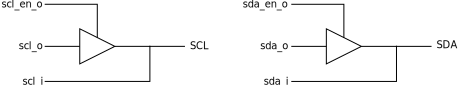
\includegraphics[width=.75\textwidth]{fig/i2c-ports}}
  \caption{Connecting the I$^2$C ports}
  \label{fig:i2c-ports}
\end{figure}

To instantiate a tri-state buffer in VHDL:

\footnotesize
\begin{verbatim}
      SCL   <= scl_o when (scl_en_o = '1') else
               'Z';
      scl_i <= SCL;

      SDA   <= sda_o when (sda_en_o = '1') else
               'Z';
      sda_i <= SDA;
\end{verbatim}

\normalsize
\noindent and in Verilog:

\footnotesize
\begin{verbatim}
      assign SCL   = (scl_en_o) ? scl_o : 1'bz;
      assign scl_i = SCL;
      assign SDA   = (sda_en_o) ? sda_o : 1'bz;
      assign sda_i = SDA;
\end{verbatim}

\normalsize

The rest of the ports should be connected in a normal manner to an external controlling module. A
component declaration of the \textit{i2c\_slave} module is readily available in the 
\textit{i2c\_slave\_pkg.vhd} package file. The package also defines constants for the 
statuses readable at the \textit{stat\_o} pin. Refer to Section~\ref{sec:oper} for details 
regarding the various statuses.

\begin{table}[h]
  \caption{Ports of \textit{i2c\_slave} module}
  \label{tbl:ports}
  \centerline
  {
    \begin{tabular}{l c p{.65\textwidth}}
      \hline
      \multicolumn{1}{c}{\textbf{Name}} & \textbf{Size} & \multicolumn{1}{c}{\textbf{Description}} \\
      \hline
      clk\_i & 1 & Clock input \\
      rst\_n\_i & 1 & Active-low reset input \\
      scl\_i & 1 & SCL line input \\
      scl\_o & 1 & SCL line output \\
      scl\_en\_o & 1 & SCL line tri-state enable \\
      sda\_i & 1 & SDA line input \\
      sda\_o & 1 & SDA line output \\
      sda\_en\_o & 1 & SDA line output tri-state enable \\
      i2c\_addr\_i & 7 & I$^2$C slave address of the module, compaired against received address \\
      ack\_n\_i & 1 & ACK to be sent to the master in case of master write transfers \\
      op\_o & 1 & State of the R/W bit at the end of the address byte \\
      tx\_byte\_i & 8 & Byte of data to be sent over I$^2$C \\
      rx\_byte\_o & 8 & Byte received over I$^2$C \\
      done\_p\_o & 1 & One \textit{clk\_i} cycle-wide pulse, signaling the slave module 
                       has performed a valid transfer \\
      stat\_o & 3 & Current state of communication \\
      \hline
    \end{tabular}
  }
\end{table}

%==============================================================================
% SEC: I2C bus
%==============================================================================
\section{I$^2$C Bus Protocol}
The I$^2$C bus protocol is a two-wire protocol defined by Philips/NXP. The original 
specification \cite{i2c-spec} defines all aspects of the protocol, from hardware 
connections on the bus, to bit- and byte-level data transfers and electrical
characteristics of the bus. A summary of the protocol is given here.

\begin{figure}[h]
  \centerline{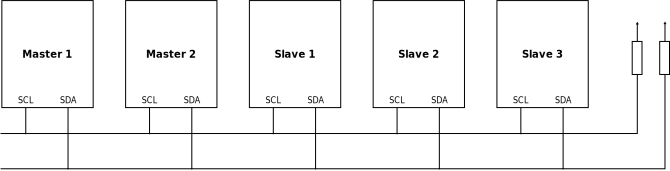
\includegraphics[width=\textwidth]{fig/i2c-bus}}
  \caption{I$^2$C bus topology}
  \label{fig:i2c-bus}
\end{figure}

Devices on the I$^2$C bus are connected together via two pins on the bus: the SCL 
(serial clock) and SDA (serial data) pins. I$^2$C masters drive the SCL line to send or
receive bits on the SDA line. Both the SCL and SDA lines on an I$^2$C device are open-collector
pins; as Figure~\ref{fig:i2c-bus} shows, one pull-up resistor on the bus connects the line to 
VCC and I$^2$C devices connect the SCL and SDA lines to ground when they drive the lines. 
In this way, a device can set a logic low level on the bus by driving the pin and a logic 
high level by releasing the pin.

A typical I$^2$C bit-level transfer (Figure~\ref{fig:i2c-bitlevel}) follows the following sequence:
\begin{itemize}
  \item master sends a start condition, driving the SDA line low while the SCL line is high
  \item master issues a series of SCL pulses to a slave to read or write bits;
  the SDA line must be stable for the duration of SCL high pulse for the bit to be properly
  transferred
  \item master sends a stop condition by releasing the SDA line while SCL line is high,
  or a repeated start (similar to start) condition if it wants to continue data transfer
\end{itemize}

\begin{figure}[h]
  \centerline{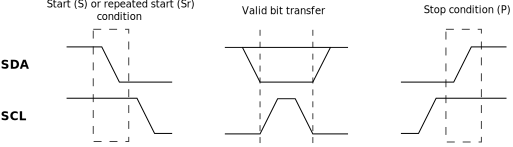
\includegraphics[width=\textwidth]{fig/i2c-bitlevel}}
  \caption{Bit-level transfers on the I$^2$C bus}
  \label{fig:i2c-bitlevel}
\end{figure}

Data are transferred on the bus in bytes, one bit at a time starting with the most significant bit.
After each sent byte, the other communicating party ACKs~('0') or NACKs~('1') the transfer on a
9$^{th}$ SCL cycle. Any number of bytes can be sent during a transfer, the master decides when data
transfer should stop by sending the stop condition. The folowing steps comprise a complete I$^2$C
data transfer (Figure~\ref{fig:i2c-transf}):
\begin{itemize}
  \item master sends start condition
  \item master sends slave address (7 bits of address + one R/W bit)
  \item if a slave with this address exists, it ACKs ('0') the master
  \item based on the R/W bit ('0' for read from  slave, '1' for write to slave), the master either
  reads or writes a byte bit by bit from/to the slave
  \item the receiver ACKs ('0') or NACKs ('1') the byte on the ninth SCL cycle
  \item any number of bytes may be sent, each followed by an ACK or NACK from the receiver
  \item \textbf{optional:} the master may (or may not) reverse data transfer by issuing a repeated start and sending the
  slave address with the R/W bit flipped
  \item \textbf{optional:} any number of bytes may be sent, each followed by an ACK or NACK from the receiver
  \item the master ends data transfer by sending the stop condition
\end{itemize}

\begin{figure}
  \centerline{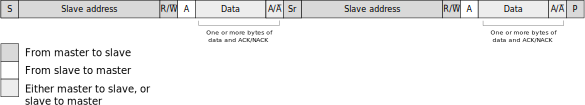
\includegraphics[width=\textwidth]{fig/i2c-transf}}
  \caption{Bytes transferred on the I$^2$C bus}
  \label{fig:i2c-transf}
\end{figure}

%==============================================================================
% SEC: Operation
%==============================================================================
\pagebreak
\section{Operation}
\label{sec:oper}

The \textit{i2c\_slave} waits for a start condition to be performed on the I$^2$C bus by a
master module. The address is shifted in and if it matches the slave address set via 
the \textit{i2c\_addr\_i} input, the \textit{done\_p\_o} output is set for one \textit{clk\_i}
cycle and the \textit{stat\_o} output signals an address match. Based on the eighth 
bit of the first I2C transfer byte, the module then starts shifting in or out each byte 
in the transfer, setting the \textit{done\_p\_o} output for one clock cycle after each 
received/sent byte. The \textit{stat\_o} output can be checked to see if the byte has been 
sent/received correctly.

When the cycle-wide \textit{done\_p\_o} output is high (after every successful transfer, or a
stop condition) the \textit{stat\_o} (possibly together with the \textit{op\_o}) output can be checked
to see the appropriate action to be taken. The various statuses possible at the
\textit{stat\_o} output are listed in Table~\ref{tbl:stat}.

\begin{table}[h]
  \caption{Statuses at the \textit{stat\_o} pin}
  \label{tbl:stat}
  \centerline
  {
    \begin{tabular}{c p{.65\textwidth}}
      \hline
      \multicolumn{1}{c}{\textbf{\textit{stat\_o}}} & \multicolumn{1}{c}{\textbf{Description}} \\
      \hline
      00 & Slave idle, waiting for start condition. This is the state upon startup and after the I$^2$C stop
           condition is received \\
      01 & Address sent by the master matches that at \textit{i2c\_addr\_i}; \textit{op\_o}
           valid \\
      10 & Read done, waiting for ACK/NACK to send to master \\
      11 & Write done, waiting for next byte to send to master \\
      \hline
    \end{tabular}
  }
\end{table}

The \textit{ack\_n\_i} port is used for sending the ACK to the master. The polarity of the bit
is that of the I$^2$C ACK signal ('0' -- ACK, '1' -- NACK). A '0' should be set
at the input also when the address is ACKed, otherwise the slave will not acknowledge its own 
address. This implies that the \textit{ack\_n\_i} pin can be used to isolate the slave from the
bus.

\subsection{Read mode}

When the eighth bit of the address byte is low (R/W = '0'), the slave goes into read
mode. Each bit of the byte sent by the master is shifted in on the falling edge of SCL. After 
eight bits have been shifted in, \textit{done\_p\_o} is set for one \textit{clk\_i} cycle and 
the status signals a successful read ("10"). The received byte should be read from the 
\textit{rx\_byte\_o} output and an ACK ('0') or NACK~('1') should be sent to the master via the
\textit{ack\_n\_i} pin. The \textit{i2c\_slave} module does not implement clock stretching, 
so the \textit{ack\_n\_i} pin should be set before the SCL line goes high.

The steps below should be followed when reading one or more bytes sent by the master:

\begin{enumerate}
  \item Wait for \textit{done\_p\_o} to go high, signaling the I$^2$C address of the slave
    has been read.
  \item Check that \textit{stat\_o} is "01" (address good) and that \textit{op\_o} is '0' 
    (master write, slave read). Set a '0' at the \textit{ack\_n\_i} input to send the 
    ACK to the address; if \textit{ack\_n\_i} is '1', the slave does not acknowledge its 
    own address.
  \item Wait for \textit{done\_p\_o} to go high.
  \item Check that \textit{stat\_o} is "10" (read done), read the received byte from
    \textit{rx\_byte\_o} and write a '0' at \textit{ack\_n\_i} to send an ACK, or a
    '1' to send an NACK.
  \item The transfer is repeated until the master sends a stop condition.
  \item After the stop condition is received, the \textit{done\_p\_o} goes high for one
  clock cycle and the status is set to "00".
\end{enumerate}

\subsection{Write mode}

When a master reads from the slave, the eighth bit of the address byte is high 
(R/W = '1'). In this case, the \textit{i2c\_slave} module goes in write mode, where
the byte at the \textit{tx\_byte\_i} port is sent to the master. When the byte has been
successfully sent, the \textit{done\_p\_o} is high for one clock cycle and the \textit{stat\_o}
port has the value "11", signaling the slave has successfully sent a byte and is
awaiting the loading of another byte.

The steps below should be followed when writing one or more bytes to a master:

\begin{enumerate}
  \item Wait for \textit{done\_p\_o} to go high, signaling the I$^2$C address of the slave
    has been read.
  \item Check that \textit{stat\_o} is "01" (address good) and \textit{op\_o} is '1' 
    (master read, slave write). Set the byte to be sent to the master at the 
    \textit{tx\_byte\_i} input. Set a '0' at \textit{ack\_n\_i} to send the ACK to the address; 
    if \textit{ack\_n\_i} is '1', the slave does not acknowledge its own address.
  \item Wait for \textit{done\_p\_o} to go high.
  \item Check that \textit{stat\_o} is "11" (write done) and set the next byte to be
    sent at the \textit{tx\_byte\_i} port.
  \item If the master acknowledges the transfer, the next byte is sent, otherwise, the master
    will send a stop condition, so the \textit{i2c\_slave} module is reset.
\end{enumerate}

Note that if a stop condition is received from the master, the \textit{done\_p\_o} goes high for
one clock cycle and the status is set to "00".

%==============================================================================
% SEC: Implementation
%==============================================================================
\section{Implementation}
\label{sec:implem}

This section presents implementation details of the \textit{i2c\_slave} module. A simplified
block diagram of the module is presented in Figure~\ref{fig:i2c-slave-bd}.

\begin{figure}[h]
  \centerline{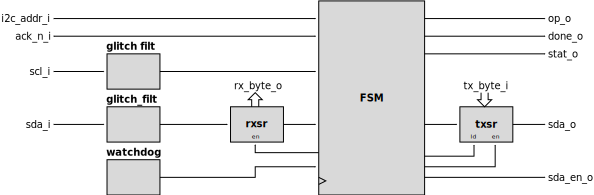
\includegraphics[width=\textwidth]{fig/i2c-slave-bd}}
  \caption{Block diagram of \textit{i2c\_slave} module}
  \label{fig:i2c-slave-bd}
\end{figure}

Deglitched versions of the SCL and SDA lines control operation of the central finite-state
machine (FSM), which sets the outputs and controls the rest of the components in the module.

The FSM is sensitive to start and stop conditions and falling edges of the SCL line. It
controls how outputs are set, when the reception and transmission shift registers (RXSR/TXSR)
are loaded and when they shift, and acknowledging to the address and bytes sent by the
master. Table~\ref{tbl:fsm} lists the states of the FSM and the operations performed
in each state.

An internal watchdog counter is implemented inside the \textit{i2c\_slave} module. This counter
counts up to 1 second and is reset at the start of each state of the FSM. If the FSM stops
in one of the states because of a bus error, the watchdog resets the FSM, thereby stopping the
communication.

\begin{longtable}{l p{.7\textwidth}}
  \caption{The states of the \textit{i2c\_slave} FSM}
  \label{tbl:fsm} \\

    \hline
    \multicolumn{1}{c}{\textbf{State}} & \multicolumn{1}{c}{\textbf{Description}} \\
    \hline
    \endfirsthead
    
    \hline
    \multicolumn{1}{c}{\textbf{State}} & \multicolumn{1}{c}{\textbf{Description}} \\
    \hline
    \endhead
    
    \hline
    \endfoot
    
    \textit{IDLE} & Idle state, FSM default state after reset and the state returned to after
                    reception of a stop condition. \\
    \textit{STA}  & State reached after a start condition is received. On the falling edge
                    of SCL, the FSM transitions to \textit{ADDR} state. \\
    \textit{ADDR} & Shift in 7 address bits and R/W bit and go to \textit{ADDR\_ACK}
                    state. Each bit is shifted in on the falling edge of SCL. If the
                    received address matches, \textit{op\_o} and \textit{done\_p\_o} are set. \\
    \textit{ADDR\_ACK} & Check received address and send the ACK value at \textit{ack\_n\_i} if
                         the address corresponds to \textit{i2c\_addr\_i}. If the R/W bit is high,
                         go to \textit{RD} state, otherwise go to \textit{WR\_LOAD\_TXSR} state.
                         If received address does not match, NACK and go to \textit{IDLE}
                         state. \\
   \textit{RD} & Shift in eight bits sent by master and go to \textit{RD\_ACK} state. Each bit 
                 is shifted in on the falling edge of SCL. When eight bits have been shifted in, 
                 set \textit{done\_p\_o}. \\
    \textit{RD\_ACK} & Read \textit{ack\_n\_i} and forward it to \textit{sda\_o} (ACK/NACK
                       from external controller). If \textit{ack\_n\_i} is '0', then go back to
                       \textit{RD} state, else to \textit{IDLE} state. \\
    \textit{WR\_LOAD\_TXSR} & Load TX shift register with data at \textit{tx\_byte\_i} input 
                              and go to \textit{WR} state. \\
    \textit{WR} & Shift out the eight bits of the TXSR starting with MSB and go to 
                  \textit{WR\_ACK} state. TXSR shifts left on falling edge of SCL. When
                  eight bits have been shifted out, \textit{done\_p\_o} is set.\\
    \textit{WR\_ACK} & Read ACK bit sent by master. If '0', go back to \textit{WR} state, otherwise
                       go to \textit{IDLE} state. \\
\end{longtable}


%\pagebreak
%\begin{table}[h]
%  \caption{The states of the \textit{i2c\_slave} FSM}
%  \label{tbl:fsm}
%  \centerline
%  {
%    \begin{tabular}{l p{.7\textwidth}}
%    \hline
%    \multicolumn{1}{c}{\textbf{State}} & \multicolumn{1}{c}{\textbf{Description}} \\
%    \hline
%    \textit{IDLE} & Idle state, FSM default state after reset and the state returned to after
%                    reception of a stop condition. \\
%    \textit{STA}  & State reached after a start condition is received. On the falling edge
%                    of SCL, the FSM transitions to \textit{ADDR} state. \\
%    \textit{ADDR} & Shift in 7 address bits and R/W bit and go to \textit{ADDR\_ACK}
%                    state. Each bit is shifted in on the falling edge of SCL. If the
%                    received address matches, \textit{op\_o} and \textit{done\_p\_o} are set. \\
%    \textit{ADDR\_ACK} & Check received address and send the ACK value at \textit{ack\_n\_i} if
%                         the address corresponds to \textit{i2c\_addr\_i}. If the R/W bit is high,
%                         go to \textit{RD} state, otherwise go to \textit{WR\_LOAD\_TXSR} state.
%                         If received address does not match, NACK and go to \textit{IDLE}
%                         state. \\
%   \textit{RD} & Shift in eight bits sent by master and go to \textit{RD\_ACK} state. Each bit 
%                 is shifted in on the falling edge of SCL. When eight bits have been shifted in, 
%                 set \textit{done\_p\_o}. \\
%    \textit{RD\_ACK} & Read \textit{ack\_n\_i} and forward it to \textit{sda\_o} (ACK/NACK
%                       from external controller). If \textit{ack\_n\_i} is '0', then go back to
%                       \textit{RD} state, else to \textit{IDLE} state. \\
%    \textit{WR\_LOAD\_TXSR} & Load TX shift register with data at \textit{tx\_byte\_i} input 
%                              and go to \textit{WR} state. \\
%    \textit{WR} & Shift out the eight bits of the TXSR starting with MSB and go to 
%                  \textit{WR\_ACK} state. TXSR shifts left on falling edge of SCL. When
%                  eight bits have been shifted out, \textit{done\_p\_o} is set.\\
%    \textit{WR\_ACK} & Read ACK bit sent by master. If '0', go back to \textit{WR} state, otherwise
%                       go to \textit{IDLE} state. \\
%    \hline
%    \end{tabular}
%  }
%\end{table}

%==============================================================================
% Bibliography
%==============================================================================
\pagebreak
\bibliographystyle{ieeetr}
\bibliography{gc_i2c_slave}

\end{document}
